\section {Regression Analysis and Modeling}
\label{sec:regression}

Many designers have a need to simulate the response of the individual components in their systems to impulse and steady state inputs. When dealing with passive electronic components, the device is typically modeled as a combination of various resistors, capacitors, and inductors. The model chosen is often due to either the required accuracy or a specific characteristic of the component that needs to be modeled. When characterizing a new component, the complex frequency response is recorded and then fit to a model. In this section, a progression of regression techniques will be evaluated for their ability to fit the measured frequency response of a capacitor to a polynomial equation. Then the accuracy of various capacitor models will be explored in regards to the fit. All models will attempt to fit the capacitor impedance data shown Figure: \ref{fig:exCapData}. See Appendix: \ref{app:genModelingImages} for the code used to generate the images shown in this section.

% This figure was generated by ./scripts/modeling/plot_ExCapData.m
\begin{figure}[ht!]
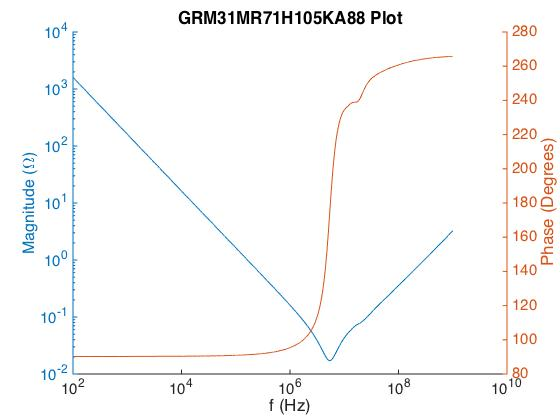
\includegraphics[keepaspectratio=true,width=6in]{./figures/modeling/exCapData.jpg}
\centering
\caption{GRM31MR71H105KA88 Capacitor Data}
\label{fig:exCapData}
\end{figure}


\subsection{Regression Analysis}
\label{sec:RegressionAnalysis}
\subsubsection{Basic LSE}
At its core, regression analysis is an optimization problem whose purpose is to fit the equation of a line to a data set. A commonly use regression analysis technique is called the Least Squares Estimate (LSE). It attempts to find a model which minimizes the squared error between an empirical set of data and itself.

The first step in applying an LSE is to choose the form of the equation that best represents the data. The equation of a line, Equation: \eqref{equ:ExLinEqu}, is chosen when only a simple linear fit is needed.
Then the squared error equation is generated, as in Equations: \eqref{equ:LSE_E2} \& \eqref{equ:LSE_E2b}.

\begin{equation}
    \label{equ:ExLinEqu}
    y = a_0 + a_1 x
\end{equation}

\begin{equation}
    \label{equ:LSE_E2}
    E^2 = \sum_{i=1}^{n} (y_i - y)^2
\end{equation}

\begin{equation}
    \label{equ:LSE_E2b}
    E^2 = \sum_{i=1}^{n} (y_i - (a_0 + a_1 x_i))^2
\end{equation}

In order to minimize the squared error over the data set, one needs to take the partial derivate of Equation: \eqref{equ:LSE_E2b} with respect to each of the unknown parameters, the coefficients, separately. While $a_0$ and $a_1$ will be constants in the final equation, they are treated as variables here until they are known. Conversely, all $x_i$ values are treated as constants. This results in Equations: \eqref{equ:LSE_PD1} \& \eqref{equ:LSE_PD2}.

\begin{align} 
    \frac{\partial E^2}{\partial a_0} &= 0 = \sum_{i=1}^{n} (-2y_i +2a_0 + 2a_1 x_i)           \label{equ:LSE_PD1} \\
    \frac{\partial E^2}{\partial a_1} &= 0 = \sum_{i=1}^{n} (-2y_i x_i +2a_0 x_i + 2a_1 x_i^2) \label{equ:LSE_PD2}
\end{align}

Up to this point most LSE analyzes follow the same basic path. But the rest of the steps depend upon the complexity of the model and solution techniques. The following steps in the basic LSE use transformations and substitutions to solve for the unknown variables. In this case case, Equation: \eqref{equ:avgb} is used to remove the summation terms from the equation.

\begin{equation}
    \label{equ:avgb} 
    \sum_{i=1}^{n} y_i  = \bar{y}n
\end{equation}

This results in Equations: \eqref{equ:LSE_sol} \& \eqref{equ:LSE_solb} with solutions shown in Equations: \eqref{equ:LSE_solc} \& \eqref{equ:LSE_sold}. The empirical data is then used to find the values of $a_0$ and $a_1$. At this point, the line can be used to estimate new points on the plot or to compare against other data sets.

\begin{equation}
    \label{equ:LSE_sol}
    0 = \bar{y} - (a_0 + 2a_1 \bar{x})
\end{equation}

\begin{equation}
    \label{equ:LSE_solb}
    0 = \bar{xy} - (a_0 \bar{x} + 2a_1 \bar{x^2})
\end{equation}

\begin{equation}
    \label{equ:LSE_solc}
    a_0 = \bar{y} - a_1 \bar{x}
\end{equation}

\begin{equation}
    \label{equ:LSE_sold}
    a_1 = \frac{\bar{xy} - \bar{x}\bar{y}}{\bar{x^2} - \bar{x}^2}
\end{equation}

An example of this type of fit can be seen in Figure: \ref{fig:basicLSE}.
\begin{figure}[ht!]
\ifisPPT
\noindent\makebox[\textwidth]{\includegraphics[keepaspectratio=true,width=\paperwidth]{../figures/regression/basicLSE.jpg}}
\else
\includegraphics[keepaspectratio=true,width=6in]{./figures/regression/basicLSE.jpg}
\fi
\centering
\caption{Basic LSE}
\label{fig:basicLSE}
\end{figure}



\subsubsection{Levy's Technique - Complex Curve Fitting}
While the basic LSE technique is sufficient for many circumstances, it is not directly applicable in situations where one needs to fit a model to a complex line, such as a transfer function. Levy \cite{levy} shows an extension of the simple LSE example that is valid for a generic polynomial transfer function. This method is important because it not only allows for a complex-valued transfer function, but it also prevents the necessity of needing to rederive the system of equations for each new model. 

\begin{equation}
    \label{equ:levy_Gs}
    G(s) = \frac{A_0 + A_1 s + A_2 s^2 + ... + A_n s^n}{B_0 + B_1 s + B_2 s^2 + ... + B_m s^m}
    ~\cite{levy}[Eq.~3]
\end{equation}

Using Equation: \eqref{equ:levy_Gs} as the generic model, Levy shows that you can use Equations: \eqref{equ:Levy_L}, \eqref{equ:Levy_S}, \eqref{equ:Levy_T}, \& \eqref{equ:Levy_U} to simplify the series of partial derivatives into a single matrix multiplication equation shown in \eqref{equ:Levy_Ans}, \eqref{equ:Levy_M}, \eqref{equ:Levy_N}, \& \eqref{equ:Levy_C}.

\begin{equation}
    \label{equ:Levy_L}
    \lambda _h = \sum_{k=0}^{m} \omega _k ^h
    ~\cite{levy}[Eq.~15]
\end{equation}

\begin{equation}
    \label{equ:Levy_S}
    S_h = \sum_{k=0}^{m} \omega _k ^h R_k
    ~\cite{levy}[Eq.~16]
\end{equation}

\begin{equation}
    \label{equ:Levy_T}
    T_h = \sum_{k=0}^{m} \omega _k ^h I_k
    ~\cite{levy}[Eq.~17]
\end{equation}

\begin{equation}
    \label{equ:Levy_U}
    U_h = \sum_{k=0}^{m} \omega _k ^h (R_k ^2 + I_k ^2)
    ~\cite{levy}[Eq.~18]
\end{equation}

\begin{equation}
    \label{equ:Levy_Ans}
    MN = C
    ~\cite{levy}[Eq.~20]
\end{equation}

\setcounter{MaxMatrixCols}{12} % Allows each row of M to fit on one line
\begin{equation}
\label{equ:Levy_M}
M = 
\begin{bmatrix}
\lambda _0 & 0          & -\lambda _2 &  0           & \lambda _4  & \cdots &  T_1    & S_2    & -T_3   & -S_4   &  T_5    & \cdots \\
0          & \lambda _2 & 0           & -\lambda _4  & 0           & \cdots & -S_2    & T_3    &  S_4   & -T_5   & -S_6    & \cdots \\
\lambda _2 & 0          & -\lambda _4 &  0           & \lambda _6  & \cdots &  T_3    & S_4    & -T_5   & -S_6   &  T_7    & \cdots \\
0          & \lambda _4 & 0           & -\lambda _6  & 0           & \cdots & -S_4    & T_5    &  S_6   & -T_7   & -S_8    & \cdots \\

\vdots     & \vdots     &  \vdots     & \vdots       & \vdots      &        &  \vdots & \vdots & \vdots & \vdots &  \vdots &        \\ 
T_1        & -S_2       & -T_3        &  S_4         & T_5         & \cdots &  U_2    & 0      & -U_4   &  0     &  U_6    & \cdots \\
S_2        &  T_3       & -S_4        & -T_5         & S_6         & \cdots &  0      & U_4    &  0     & -U_6   &  0      & \cdots \\
T_3        & -S_4       & -T_5        &  S_6         & T_7         & \cdots &  U_4    & 0      & -U_6   &  0     &  U_8    & \cdots \\
\vdots     & \vdots     &  \vdots     & \vdots       & \vdots      & \vdots &  \vdots & \vdots & \vdots & \vdots &  \vdots &        \\ 
\end{bmatrix}
~\cite{levy}[Eq.~21a]
\end{equation}

\begin{multicols}{2}
    \begin{equation}
        \label{equ:Levy_N}
        N = 
        \begin{bmatrix}
            A_0 \\
            A_1 \\
            A_2 \\
            A_3 \\
            \vdots \\
            B_1 \\
            B_2 \\
            B_3 \\
            \vdots
        \end{bmatrix}
        ~\cite{levy}[Eq.~21b]
    \end{equation}

    \begin{equation}
        \label{equ:Levy_C}
        C = 
        \begin{bmatrix}
            S_0 \\
            T_1 \\
            S_2 \\
            T_3 \\
            \vdots \\
            0   \\
            U_2 \\
            0   \\
            \vdots
        \end{bmatrix}
        ~\cite{levy}[Eq.~21c]
    \end{equation}
\end{multicols}

Levy's technique works well for applications where there is a small dynamic frequency range and a small number of coefficients, but there a several problems with it.
The first problem is that for models with a wide bandwidth, the solution to Equation: \eqref{equ:Levy_Ans}, involves an ill-conditioned matrix. This means that the solution to the system of equations will experience precision errors.
The second problem is that this technique favors the magnitude plot at the high frequency range. As can be seen in Figure: \ref{fig:levy}, a applying Levy's technique with $3^{rd}$ order model provides an unuseable fit to the emperical data.

% Run /scripts/regression/run_levy_iter.m with NumDeg = 3, DenDeg = 3, and iterations = 1.
\begin{figure}[ht!]
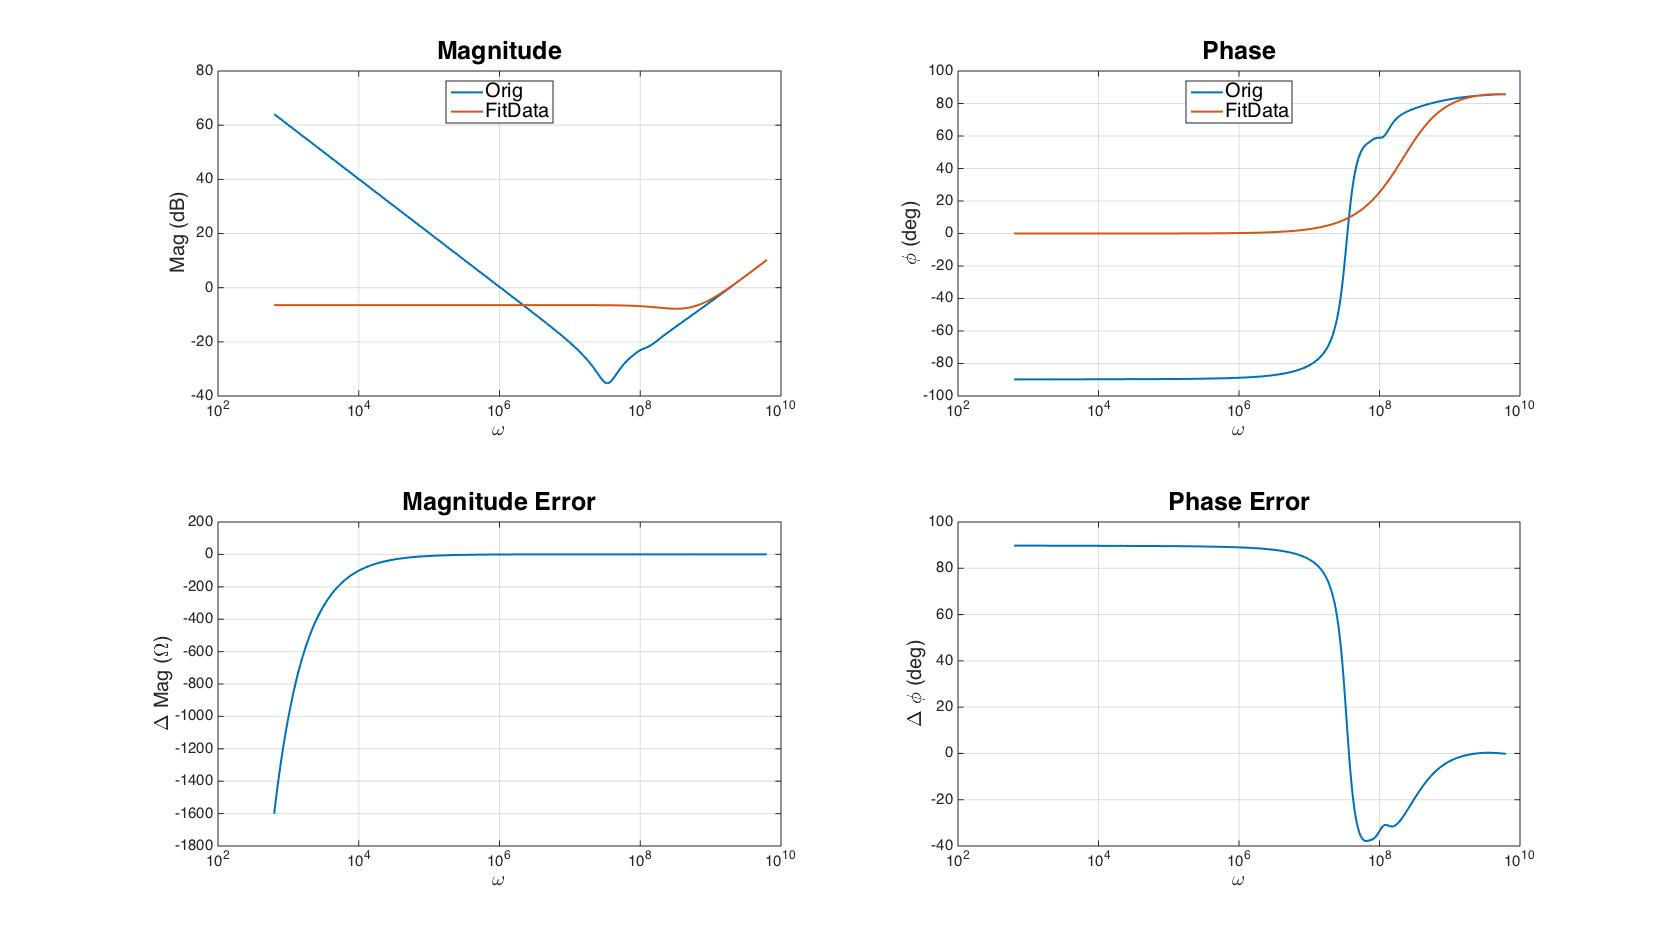
\includegraphics[keepaspectratio=true,width=6in]{./figures/regression/levy.jpg}
\centering
\caption{Levy's Technique}
\label{fig:levy}
\end{figure}



\subsubsection{Weighted LSE}
\label{sec:weightedLSE}
One improvement that can be made upon Levy's method is to iterate with a frequency dependent weighting function until the error term is minimized \cite{levy_iter}. By multiplying Levy's error function by the weighting term in Equation: \eqref{equ:iter_Weight}, we get Equation: \eqref{equ:iter_Err}, which can be minimized to obtain a new system of equations.
The $L$ subscript stands for the current iteration, while $L-1$ stands for the previous iteration.

\begin{equation}
    \label{equ:iter_Weight}
    W_{kL} = \frac{1}{|Q(jw_k)_{L-1}|^2}
    ~\cite{levy_iter}
\end{equation}

\begin{equation}
    \label{equ:iter_Err}
    E = \sum_{k=1}^{n} |\epsilon _k ^{'}|^2W_{kL}
    ~\cite{levy_iter}[Eq.~7]
\end{equation}

Equations \eqref{equ:Levy_Ans}, \eqref{equ:Levy_M}, \eqref{equ:Levy_N}, \& \eqref{equ:Levy_C} are the same, with Equations \eqref{equ:Levy_L}, \eqref{equ:Levy_S}, \eqref{equ:Levy_T}, \& \eqref{equ:Levy_U} being replaced with Equations: \eqref{equ:Iter_L}, \eqref{equ:Iter_S}, \eqref{equ:Iter_T}, \& \eqref{equ:Iter_U}.

\begin{equation}
    \label{equ:Iter_L}
    \lambda _h = \sum_{k=0}^{m} \omega _k ^hW_{kL}
    ~\cite{levy_iter}[Eq.~9]
\end{equation}

\begin{equation}
    \label{equ:Iter_S}
    S_h = \sum_{k=0}^{m} \omega _k ^h R_kW_{kL}
    ~\cite{levy_iter}[Eq.~10]
\end{equation}

\begin{equation}
    \label{equ:Iter_T}
    T_h = \sum_{k=0}^{m} \omega _k ^h I_kW_{kL}
    ~\cite{levy_iter}[Eq.~11]
\end{equation}

\begin{equation}
    \label{equ:Iter_U}
    U_h = \sum_{k=0}^{m} \omega _k ^h (R_k ^2 + I_k ^2)W_{kL}
    ~\cite{levy_iter}[Eq.~12]
\end{equation}

Dependent upon the initial conditons and the model order, this particular method is not gauranteed to converge. Figure: \ref{fig:levyIter_Err1} was generated with an initial condition of $Q(jw_k) == 1$ and a model order of 7. It shows that, for this data set, the squared error of the magnitude and phase do not converge after a particular number of iterations. Furthermore, they do not reach their minimums at the same iteration. In order to select the desired iteration, the magnitude and phase squared plots are normalized as in Equation: \eqref{equ:ErrMin}. The index of the minimum of Figure: \ref{fig:levyIter_Err1} is selected as the best fit.

\begin{equation}
\label{equ:ErrMin}
n = min(Emag/max(eMag) + Epha/max(ePha))
\end{equation}

\begin{figure}[ht!]
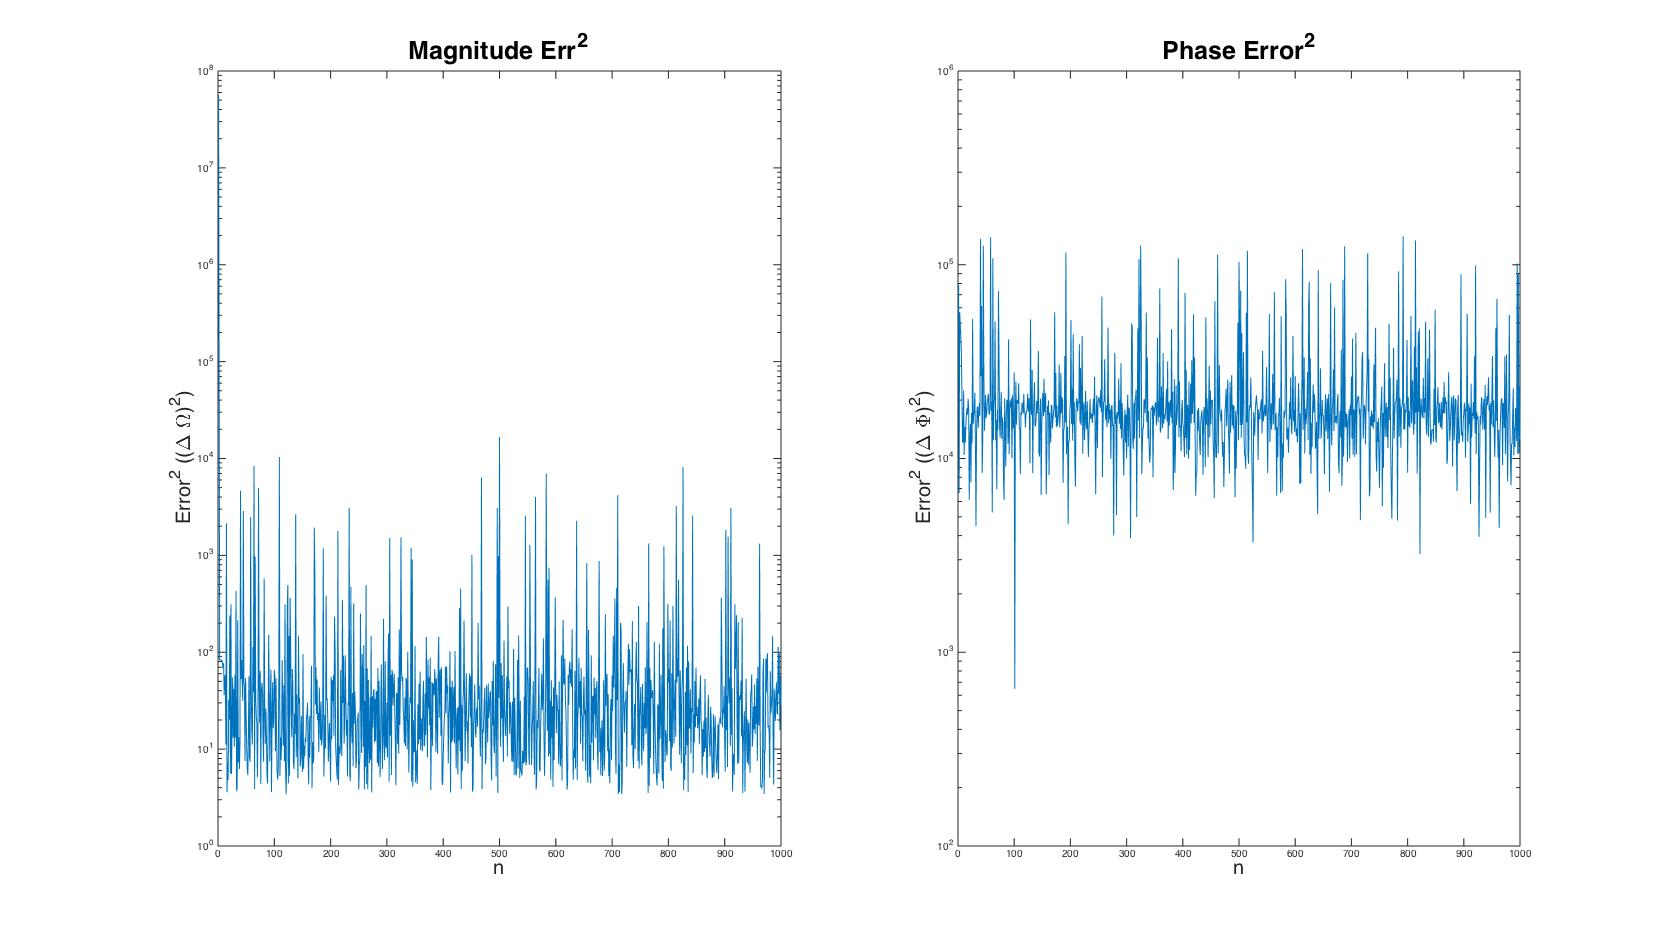
\includegraphics[keepaspectratio=true,width=6in]{./figures/modeling/levyIter_Err1.jpg}
\centering
\caption{LSE + Iteration -- Magnitude and Phase Error}
\label{fig:levyIter_Err1}
\end{figure}

% Run ./scripts/regression/run_levy_iter.m with numDeg = 7, denDeg = 7, and iterations = 100 to obtain this image.
\begin{figure}[ht!]
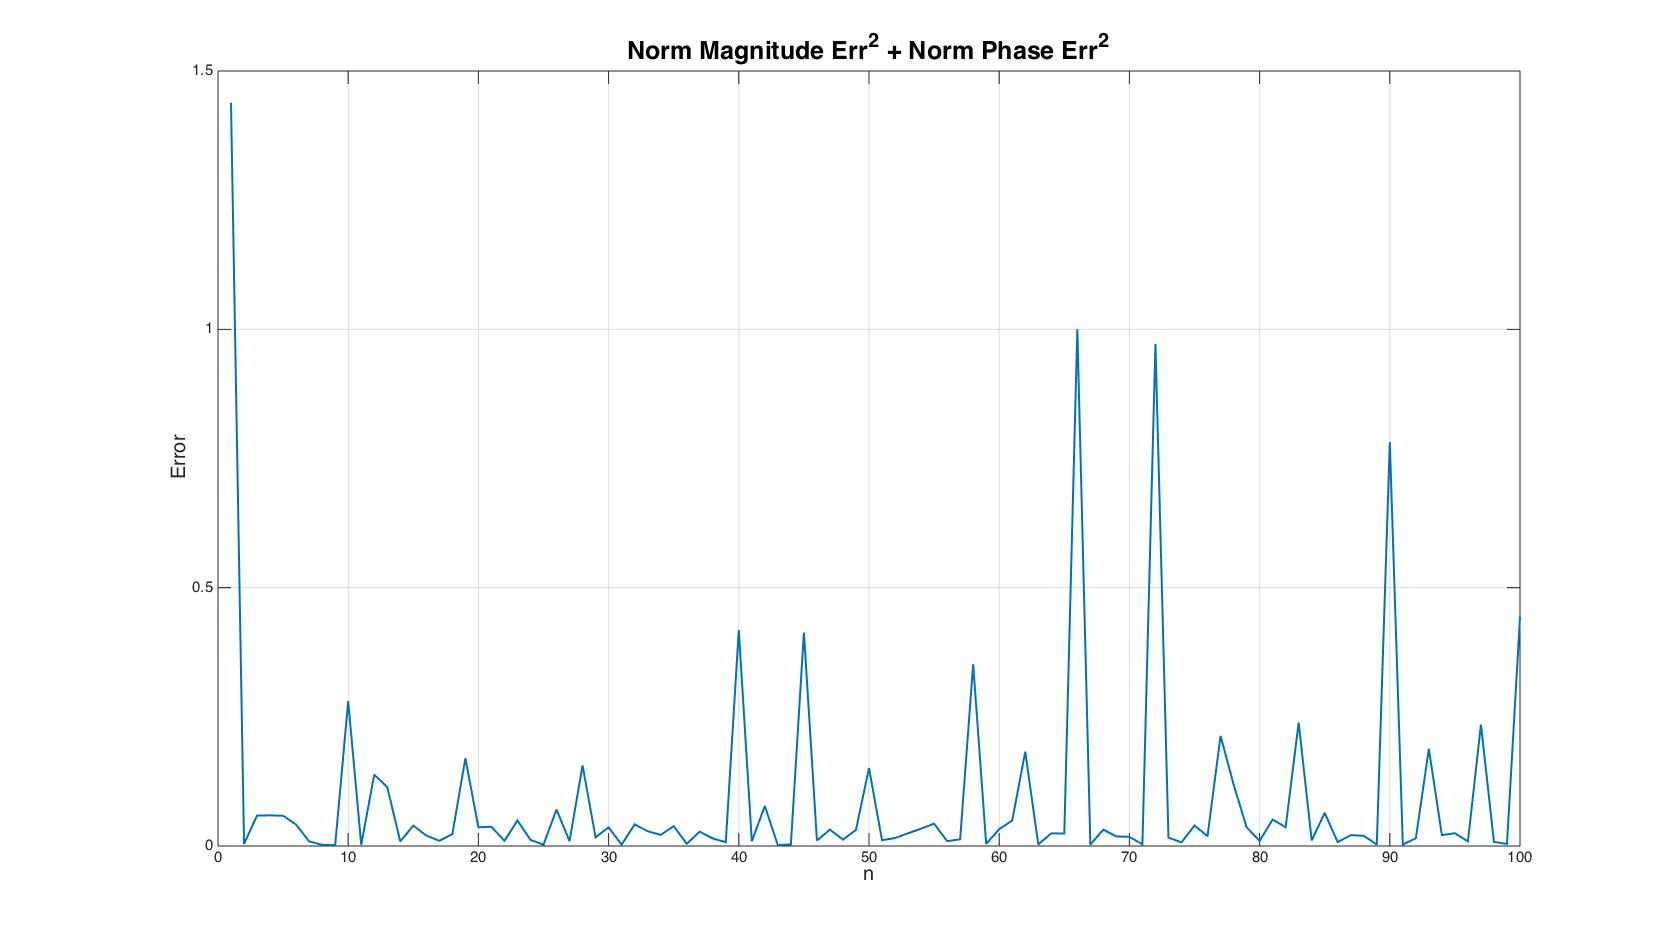
\includegraphics[keepaspectratio=true,width=6in]{./figures/regression/levyIter_Err2.jpg}
\centering
\caption{LSE + Iteration -- Combined Error}
\label{fig:levyIter_Err2}
\end{figure}



Figure: \ref{fig:levyIter} shows that this method can result in a much improved result over the Levy's original method, as seen in Figure: \ref{fig:levy}.

\begin{figure}
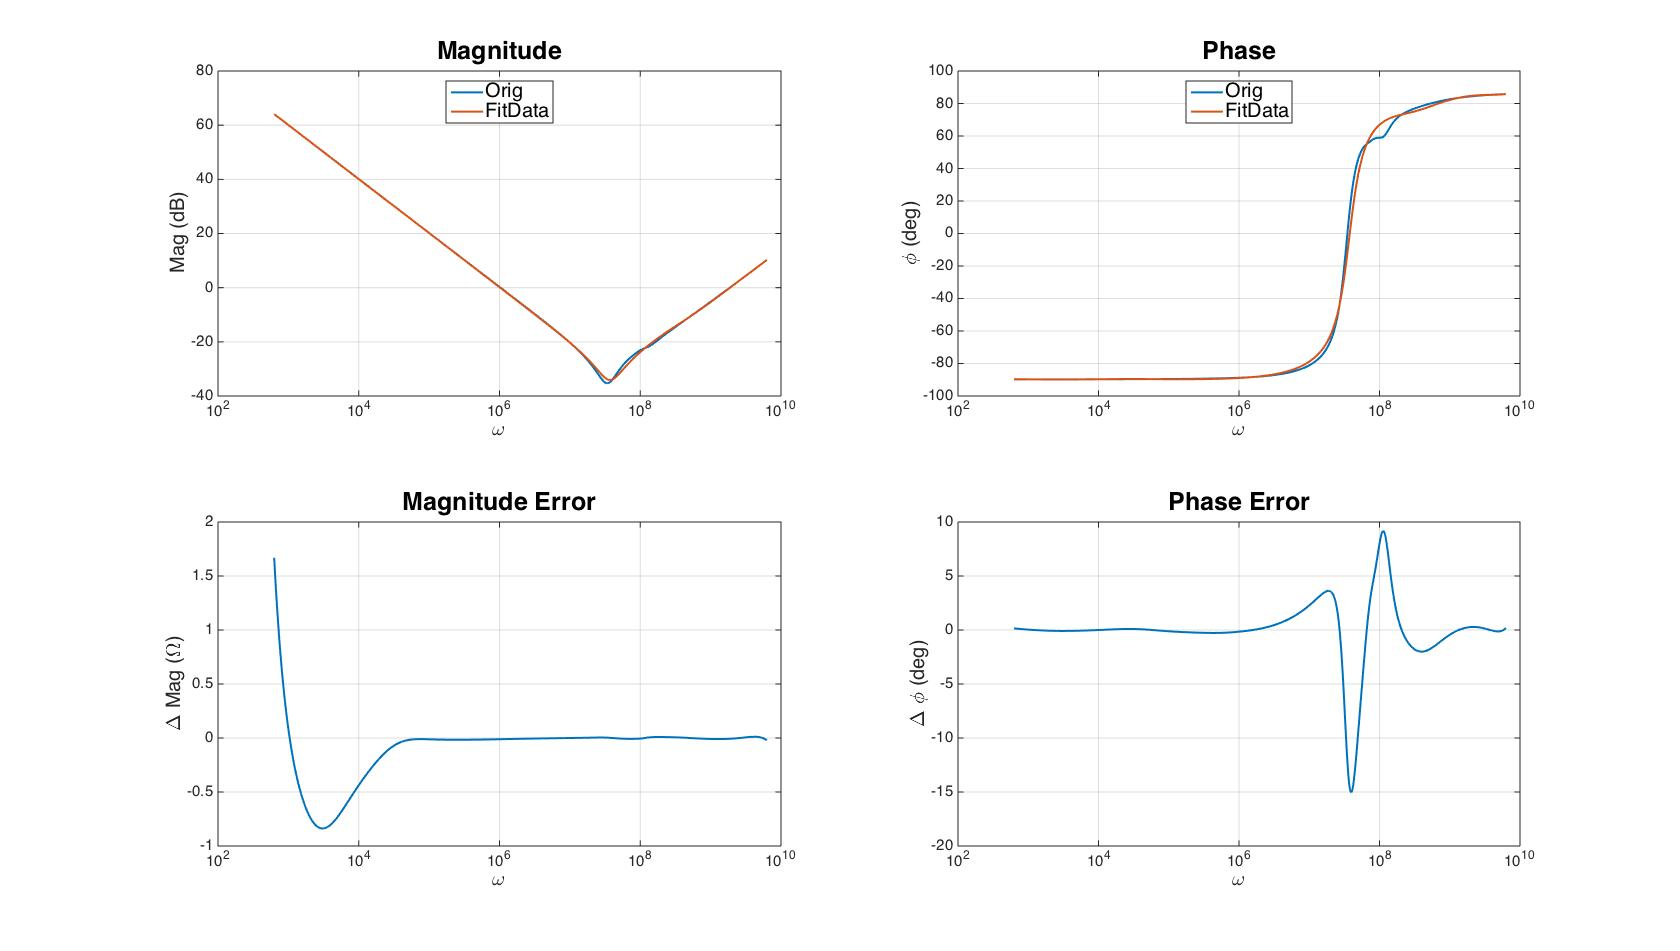
\includegraphics[keepaspectratio=true,width=6in]{./figures/modeling/levyIter.jpg}
\centering
\caption{LSE + Iteration}
\label{fig:levyIter}
\end{figure}


\subsection{Modeling}
This section will investigate several of the most common capacitor models. It will show how to fit them to a data set with Levy's method described in Section: \ref{sec:RegressionAnalysis}, and will describe their effectiveness and limitations in doing so.

\subsubsection{6 Term Model}
\begin{figure}[ht!]
\ifisPPT
\noindent\makebox[\textwidth]{\includegraphics[keepaspectratio=true,width=\paperwidth]{../figures/regression/fullModel.jpg}}
\else
\includegraphics[keepaspectratio=true,width=2in]{./figures/regression/fullModel.jpg}
\fi
\centering
\caption{6 Term Model}
\label{fig:fullModel}
\end{figure}


The model shown in Figure: \ref{fig:fullModel} shows several of the most important parameters for a capacitor. It's impedance, shown in Equation: \eqref{equ:fullModelImpedance}, can be used as the basis for a regression analysis.

\begin{equation}
    \begin{split}
        \label{equ:fullModelImpedance}
        \bar{Z}(s) = \frac{(R_E + R_L) + (L_E + C_DR_DR_E + C_DR_DR_L + CR_ER_L + C_DR_ER_L)s}{1 + (C_DR_D + CR_L + C_DR_L)s + CC_DR_DR_Ls^2} \\ 
        + \frac{(C_DL_ER_D + CL_ER_L + C_DL_ER_L + CC_DR_DR_ER_L)s^2 + CC_DL_ER_DR_Ls^3}{1 + (C_DR_D + CR_L + C_DR_L)s + CC_DR_DR_Ls^2}
    \end{split}
\end{equation}

\begin{equation}
    \label{equ:fullModelPoly}
    \bar{Z}(s) = \frac{a_0 + a_1s + a_2s^2 + a_3s^3}{b_0 + b_1s + b_2s^2}
\end{equation}


For this model, Equations: \eqref{equ:Levy_M}, \eqref{equ:Levy_N}, \& \eqref{equ:Levy_C} simplify down to Equations: \eqref{equ:fullModel_M}, \eqref{equ:fullModel_N}, \& \eqref{equ:fullModel_C}.

\begin{equation}
    \label{equ:fullModel_M}
    M = 
    \begin{bmatrix}
        \lambda _0 & 0          & -\lambda _2 & 0           &  T_1    & S_2 \\
        0          & \lambda _2 & 0           & -\lambda _4 & -S_2    & T_3 \\
        \lambda _2 & 0          & -\lambda _4 & 0           &  T_3    & S_4 \\
        0          & \lambda _4 & 0           & -\lambda _6 & -S_4    & T_5 \\
        T_1        & -S_2       & -T_3        &  S_4        &  U_2    & 0   \\
        S_2        &  T_3       & -S_4        & -T_5        &  0      & U_4
    \end{bmatrix}
\end{equation}

\begin{multicols}{2}
    \begin{equation}
        \label{equ:fullModel_N}
        N = 
        \begin{bmatrix}
            A_0 \\
            A_1 \\
            A_2 \\
            A_3 \\
            B_1 \\
            B_2
        \end{bmatrix}
    \end{equation}

    \begin{equation}
        \label{equ:fullModel_C}
        C = 
        \begin{bmatrix}
            S_0 \\
            T_1 \\
            S_2 \\
            T_3 \\
            0   \\
            U_2
        \end{bmatrix}
    \end{equation}
\end{multicols}

Using this model, the regression analysis output described in Section: \ref{sec:weightedLSE} can be seen in Figure: \ref{fig:fullModel_BadOutput}. The fit tracks the original data well, except for low frequencies and near resonance. 

\begin{figure}[ht!]
\ifisPPT
\noindent\makebox[\textwidth]{\includegraphics[keepaspectratio=true,width=\paperwidth]{../figures/regression/fullModel_BadOutput.jpg}}
\else
\includegraphics[keepaspectratio=true,width=6in]{./figures/regression/fullModel_BadOutput.jpg}
\fi
\centering
\caption{6 Term Model: Bad Initilization}
\label{fig:fullModel_BadOutput}
\end{figure}


Equations: \eqref{equ:fullModel_BadOutputCoeff} shows solution for the polynomial coefficients. Using Equations: \eqref{equ:fullModelPoly} and \eqref{equ:fullModelPoly}, the circuit parameters can be found through Equations: \eqref{equ:fullModel_CoeffEq_a0}-\eqref{equ:fullModel_CoeffEq_b2}, with the solution as seen in Equations: \eqref{equ:fullModel_BadOutputCoeff} \& \eqref{equ:fullModel_BadOutputParams}.
Even though the polynomial coefficients gave an acceptable fit to the data, it resulted in unacceptable circuit parameters. Since $C$ and $R_D$ are negative, this model is not physically realizable.

\begin{align}
     a_0 &= R_E + R_L                                         \label{equ:fullModel_CoeffEq_a0} \\
     a_1 &= L_E + C_DR_DR_E + C_DR_DR_L + CR_ER_L + C_DR_ER_L \label{equ:fullModel_CoeffEq_a1} \\
     a_2 &= C_DL_ER_D + CL_ER_L + C_DL_ER_L + CC_DR_DR_ER_L   \label{equ:fullModel_CoeffEq_a2} \\
     a_3 &= CC_DL_ER_DR_L                                     \label{equ:fullModel_CoeffEq_a3} \\
     b_0 &= 1                                                 \label{equ:fullModel_CoeffEq_b0} \\
     b_1 &= C_DR_D + CR_L + C_DR_L                            \label{equ:fullModel_CoeffEq_b1} \\
     b_2 &= CC_DR_DR_L                                        \label{equ:fullModel_CoeffEq_b2}
\end{align}

\begin{multicols}{2}
    \begin{equation}
        \label{equ:fullModel_BadOutputCoeff}
        \begin{split}
             a_0 &= 5.9991E^{+03} \\
             a_1 &= 1.7934E^{-04} \\
             a_2 &= 3.3158E^{-12} \\
             a_3 &= 6.8295E^{-22} \\
             b_0 &= 1.0000        \\
             b_1 &= 5.9057E^{-03} \\
             b_2 &= 1.4067E^{-12}
        \end{split}
    \end{equation}

    \begin{equation}
        \label{equ:fullModel_BadOutputParams}
        \begin{split}
            C &= -8.2563E^{-10} \\
            R_E &=  3.1886E^{-01} \\
            L_E &=  4.8551E^{-10} \\
            R_L &=  4.8551E^{-10} \\
            C_D &=  9.8536E^{-07} \\
            R_D &= -2.8824E^{-01}
        \end{split}
    \end{equation}
\end{multicols}

The problem comes with the author's \cite{levy_iter} suggestion that the initial guess for $Q(jw_k) == 1$. While an initial guess is required to calculate the weighting function during the first iteration, this particular choice causes the problem seen in Equations: \eqref{equ:fullModel_BadInputCoeff} \& \eqref{equ:fullModel_BadInputParams}. They show that this initial condition does not yield a rational solution for the circuit parameters.


\begin{multicols}{2}
    \mbox{}\vfill
    \begin{equation}
        \label{equ:fullModel_BadInputCoeff}
        \begin{split}
            &a_0 = 1 \\
            &a_1 = 1 \\
            &a_2 = 1 \\
            &a_3 = 1 \\
            &b_0 = 1 \\
            &b_1 = 0 \\
            &b_2 = 0
        \end{split}
    \end{equation}

    \mbox{}\vfill
    \columnbreak

    \mbox{}\vfill
    \begin{equation}
        \label{equ:fullModel_BadInputParams}
        \begin{split}
             C   &= INF \\
             R_E &= INF \\
             L_E &= INF \\
             R_L &= IND \\
             C_D &= IND \\
             R_D &= IND \\
        \end{split}
    \end{equation}
    \mbox{}\vfill
\end{multicols}



If we instead start with the rational set of circuit parameters seen in Equation: \eqref{equ:fullModel_GoodInputParams}, the starting coefficients are as seen in Equation: \eqref{equ:fullModel_GoodInputCoeff}.

\begin{multicols}{2}
    \mbox{}\vfill
    \begin{equation}
        \label{equ:fullModel_GoodInputCoeff}
        \begin{split}
             a_0 &= 2 \\
             a_1 &= 5 \\
             a_2 &= 4 \\
             a_3 &= 1 \\
             b_0 &= 1 \\
             b_1 &= 3 \\
             b_2 &= 1
        \end{split}
    \end{equation}

    \mbox{}\vfill
    \columnbreak

    \mbox{}\vfill
    \begin{equation}
        \label{equ:fullModel_GoodInputParams}
        \begin{split}
             C   &= 1 \\
             R_E &= 1 \\
             L_E &= 1 \\
             R_L &= 1 \\
             C_D &= 1 \\
             R_D &= 1 \\
        \end{split}
    \end{equation}
    \mbox{}\vfill
\end{multicols}

\begin{figure}[ht!]
\ifisPPT
\noindent\makebox[\textwidth]{\includegraphics[keepaspectratio=true,width=\paperwidth]{../figures/regression/fullModel_GoodOutput.jpg}}
\else
\includegraphics[keepaspectratio=true,width=6in]{./figures/regression/fullModel_GoodOutput.jpg}
\fi
\centering
\caption{6 Term Model: Good Initilization}
\label{fig:fullModel_GoodOutput}
\end{figure}


Figure: \ref{fig:fullModel_GoodOutput} shows a good fit across the frequency spectrum for both magnitude and phase. The model does deviate at resonance, but that is unsurprising, as the number of parameters in the model is fairly low.

